%!TEX root = ../../../adrien_gomar_phd.tex

\subsection{Numerical setup}
\label{sub:dream_ls_ael_numerical}

Two structural modes are considered for the aeroelastic study of this 
configuration: the second bending/flexion mode and the first torsion mode
of the front rotor.
The shape of the modes is shown in Fig.~\ref{fig:dream_ls_ael_modes}
with an arbitrary amplitude that allows the visualization.
Two inflection lines are seen for the 2F mode, while only
one is seen for the 1T, hence its designation.
\begin{figure}[htp]
  \centering
  \subfigure[2F]{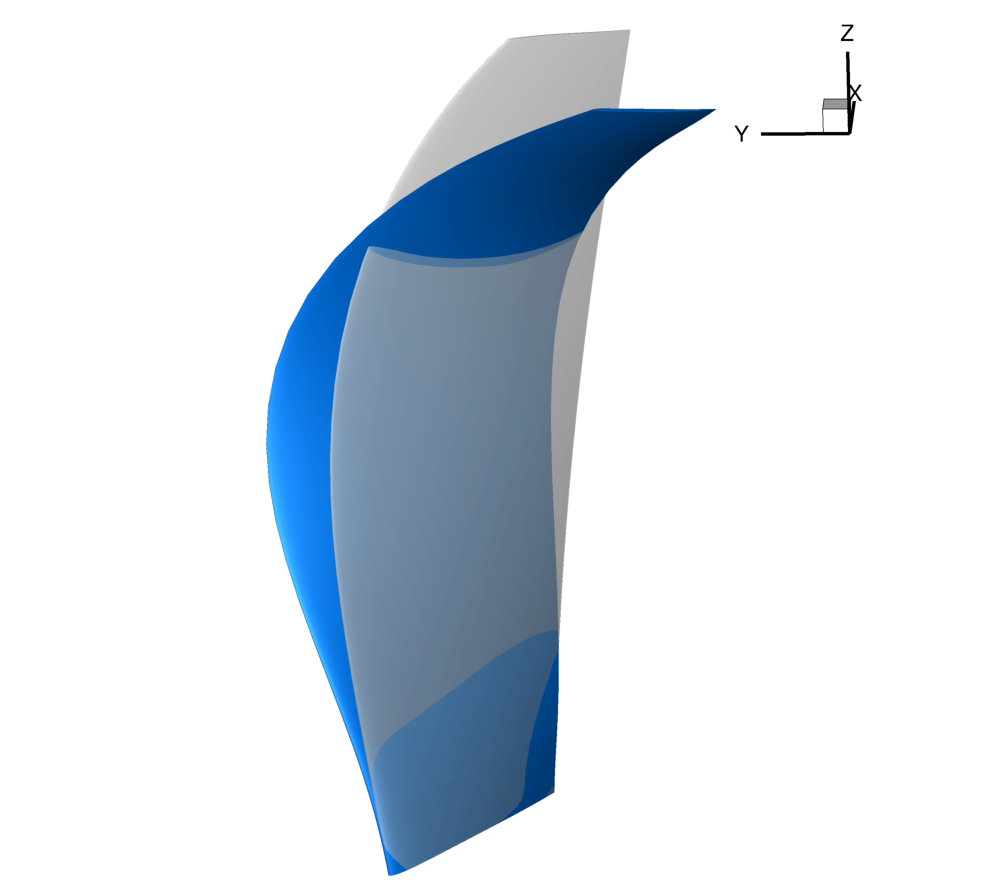
\includegraphics[height=.35\textwidth]{mode_2F.png}}
  \subfigure[1T]{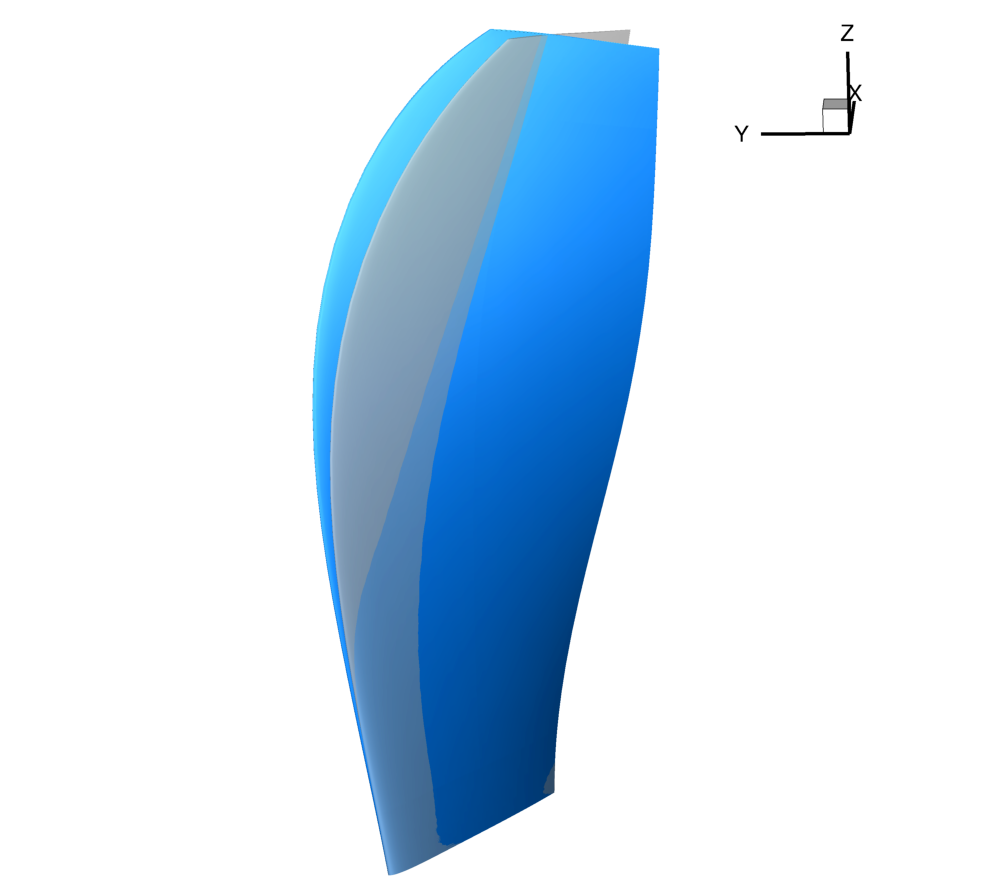
\includegraphics[height=.35\textwidth]{mode_1T.png}}
  \caption{Low-speed isolated configuration: structural modes considered.}
  \label{fig:dream_ls_ael_modes}
\end{figure}

Four nodal diameters are considered, corresponding to IBPA
values: $[-60^\circ, -30^\circ, 30^\circ, 60^\circ]$. The frequency
considered for theses modes are not correlated with the blade
passing frequency of the rear rotor. Therefore, to simulate such
a configuration using the harmonic balance approach, the
multi-frequential framework should be adopted. The ratio of the
blade passing frequency $f_{BPF}$ of rear rotor (the one that is
seen by the front rotor, see Sec.~\ref{sec:cror_unsteady})
over the frequency of the mode considered is reported in
Tab.~\ref{tab:dream_ls_ael_freq_bpf}. 

\begin{table}[htp]
  \ra{1.3} \centering
  \begin{tabular}{r|cc}
    \toprule
    &  mode 2F (IBPA $30^\circ$/$60^\circ$) & mode 1T (IBPA $30^\circ$/$60^\circ$) \\
    \midrule
    $f_{BPF} / f_{AEL}$ & 3.87/3.85 & 3.20/3.17 \\ 
    $\kappa (E)$, EVE~2N+1 & 31.3/29.2 & 1.68/1.84 \\
    $\kappa (E)$, OPT & 1.01/1.07 & 1.02/1.08 \\
    \bottomrule
  \end{tabular}
  \caption{Low-speed isolated configuration:}
  \label{tab:dream_ls_ael_freq_bpf}
\end{table} 

not correlated to the blade
passing frequency of the configuration. The multi-frequential
formulation of the harmonic balance approach is used 
(see Appendix~\ref{app:elsa}). 